%----------------------------------------------------
% Setup Beamer
%----------------------------------------------------
\documentclass[hyperref={colorlinks=true}]{beamer}

%----------------------------------------------------
% Packages to use
%----------------------------------------------------
\input{../packages.sty}

%\usetikzlibrary{external}
%\tikzexternalize % activate!

%----------------------------------------------------
% Setup Theme
%----------------------------------------------------
\input{../theme.sty}

%----------------------------------------------------
% Table of Contents at each section transition
%----------------------------------------------------

\AtBeginSection[]
{
   \begin{frame}
       \frametitle{Outline}
       \setcounter{tocdepth}{2}
       \tableofcontents[currentsection]
   \end{frame}
}

%----------------------------------------------------
% Colors
%----------------------------------------------------
\input{../mycolors.sty}

%----------------------------------------------------
% Style, formatting, and new commands
%----------------------------------------------------
\newcommand{\CourseYear}   {2024}
\newcommand{\CanvasURL}    {https://canvas.uchicago.edu/courses/58627}
\newcommand{\CanvasLink}   {\href{\CanvasURL}{\CanvasURL}}
\newcommand{\GitHubURL}    {https://github.com/UChicagoPhysics/PHYS250}
\newcommand{\GitHubLink}   {\href{\GitHubURL}{\GitHubURL}}
\newcommand{\PlatformURL}  {https://binderhub.pile.uchicago.edu/}
\newcommand{\PlatformLink} {\href{\PlatformURL}{\PlatformURL}}
\newcommand{\PiazzaURL}    {https://canvas.uchicago.edu/courses/58627/discussion\_topics}
\newcommand{\PiazzaLink}   {\href{\PiazzaURL}{\PiazzaURL}}
\input{../newcommands.sty}
\input{../EandMcommands.sty}

%----------------------------------------------------
% Set paths for plots and images
%----------------------------------------------------
\input{../paths.sty}

%----------------------------------------------------
% SETTINGS FOR THIS LECTURE
%----------------------------------------------------
\newcommand{\lecnum }  {Lecture 16}
\newcommand{\lecdate}  {November 29, 2024}
\newcommand{\topic}    {Neural Networks -- Part II}

%-----------------------------------------------------------------------------------------
% Title: [Column]{Title}
%-----------------------------------------------------------------------------------------
\title[PHYS 250 (Autumn 2024) -- \lecnum]{\topic}

%-----------------------------------------------------------------------------------------
% SubTitle: [Column]{Subtitle}
%-----------------------------------------------------------------------------------------
\subtitle{PHYS 250 (Autumn 2024) -- \lecnum}

%-----------------------------------------------------------------------------------------
% Author: [SubAuthor]{Author}
%-----------------------------------------------------------------------------------------
\author[D.W.~Miller]{David Miller}

%----------------------------------------------------
% Institute: [SubInst]{Institute}
%----------------------------------------------------
\institute[EFI, Chicago] 
{
  Department of Physics and the Enrico Fermi Institute\\
  University of Chicago
}

%----------------------------------------------------
% Institute: [SubInst]{Institute}
%----------------------------------------------------
\date[\lecdate]{\lecdate}

\subject{PHYS 250 Lecture}

\begin{document}

%==========================================================================================
% TITLE PAGE
%==========================================================================================

{
\begin{frame}
  \titlepage
\end{frame}
}

%==========================================================================================
\section[Reminders]{Reminders}
%==========================================================================================

%-----------------------------------------------------------------------------------------
\subsection[Reminders from Lecture 15]{Reminders from Lecture 15}
%-----------------------------------------------------------------------------------------

\begin{frame}%[shrink=10]
  \frametitle{Reminders from last time}

  We embarked on a whirlwind introduction to neural networks.
  
  \vspace{0.3cm}
  
  \begin{ucblock}{Neural networks and machine learning}
    \begin{itemize}
      \item \bluebf{Context and perspective} 
      \begin{itemize}
        \item We discussed the general issue of training computers to \textbf{discover, identify, and analyze patterns} of interest in datasets
        \item Categorized tasks that make use of this idea: \textbf{classification, regression, generation, clustering, anomaly detection}
      \end{itemize}
      \item \bluebf{Neural networks as a tool} 
      \begin{itemize}
        \item Introduced both the \textbf{modeling} perspective as well as the \textbf{biological} perspective on what a neural network achieves 
        \item Described the \textbf{structure and function} of a neuron
        \item Began discussing the \textbf{mathematical properties} of a neural network
      \end{itemize}
    \end{itemize}
  \end{ucblock}
  
  \mysp
  
  Today we will build our own networks! But first, I just wanted to follow-up on some points and questions from last time.

\end{frame}

%==========================================================================================
\section[Historical perspective]{Historical perspective}
%==========================================================================================

%-----------------------------------------------------------------------------------------
\subsection[Brief History of Machine Learning Generally]{Brief History of Machine Learning Generally}
%-----------------------------------------------------------------------------------------

\begin{frame}%[shrink=10]
  \frametitle{Brief history of machine learning}

  Taken from \href{http://innovationobservatory.com/node/243}{Harry Ide on InnovationLaboratory.com (18 May 2018)}:
  
  \begin{figure}
    \centering
    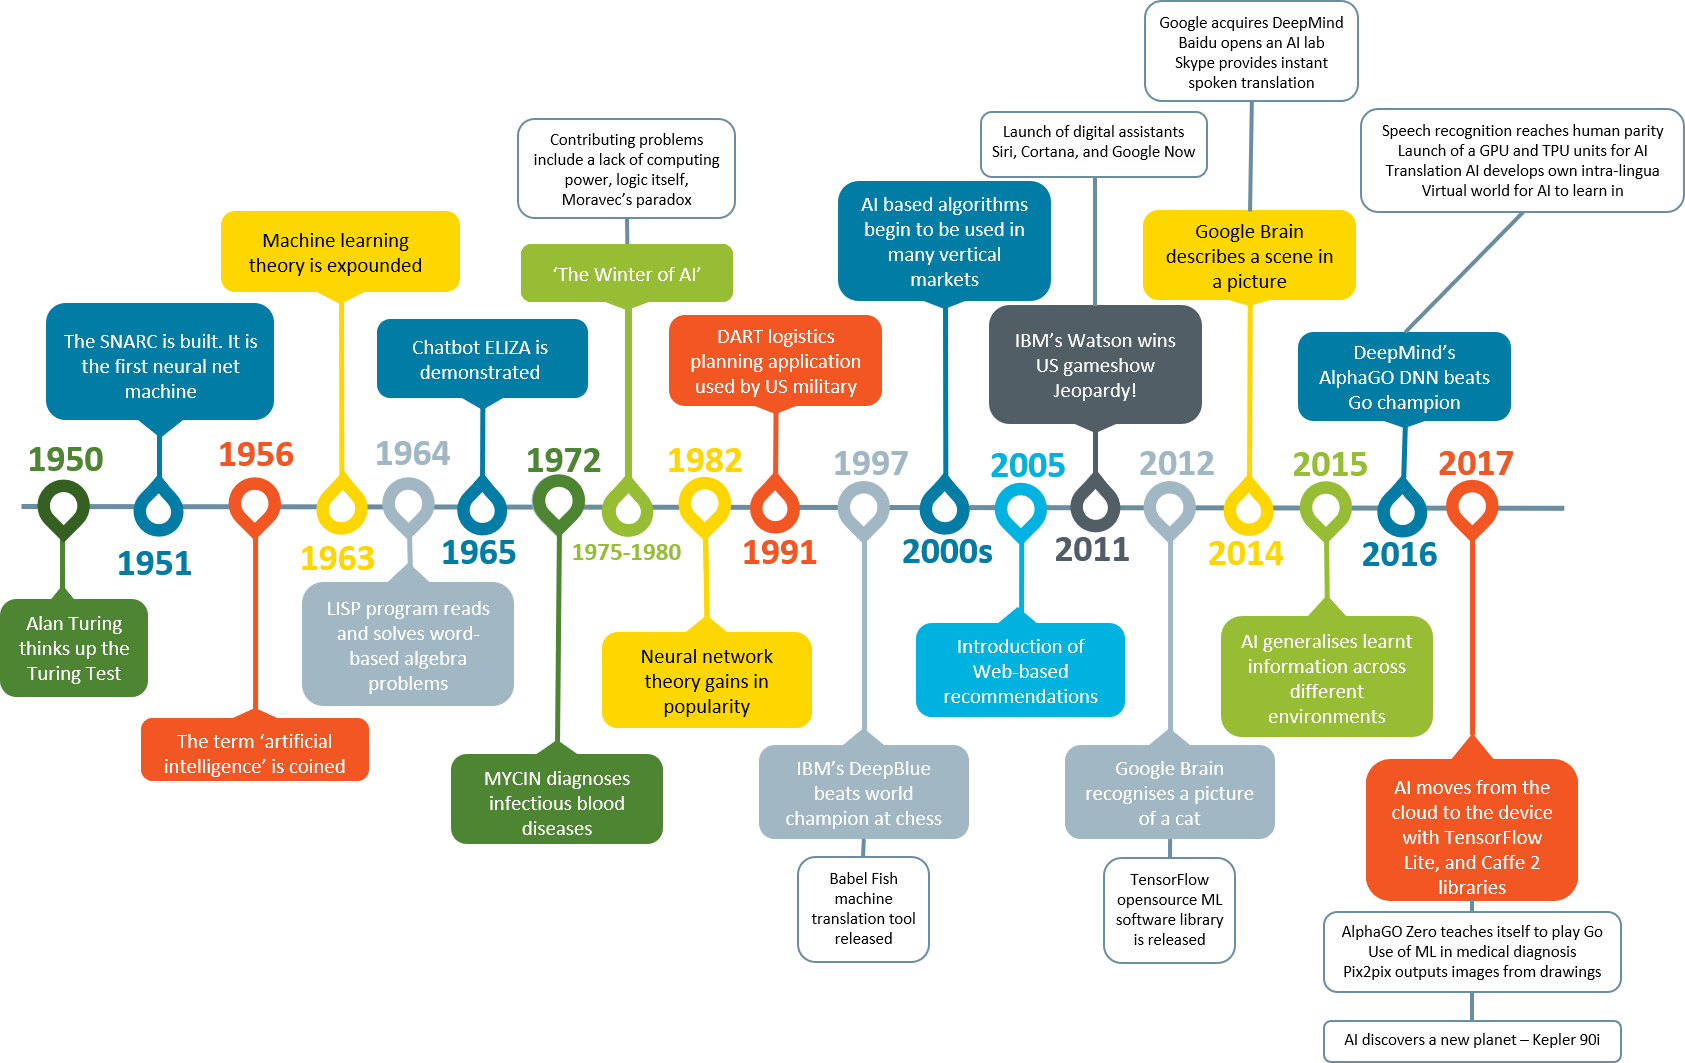
\includegraphics[width=\textwidth]{MLBreakthroughs-Timeline-to-2017.png}
  \end{figure}
  
  \only<2>{
    \begin{textblock}{12}(1.5,-8)
    \begin{ucblock}{Quote from Harry Ide on ``AI''}
      \textit{``The cutting edge might not be as sharp as many believe. AI has a nearly 70-year long history with some surprising backtracks and re-emergences among it.''}
    \end{ucblock}
    \end{textblock}
  }
\end{frame}


%-----------------------------------------------------------------------------------------
\subsection[Brief History of Neural Networks]{Brief History of Neural Networks}
%-----------------------------------------------------------------------------------------

\begin{frame}%[shrink=10]
  \frametitle{Brief history of neural networks}

  Taken from \href{https://www.slideshare.net/deview/251-implementing-deep-learning-using-cu-dnn/4}{this talk on SlideShare}:
  
  \begin{figure}
    \centering
    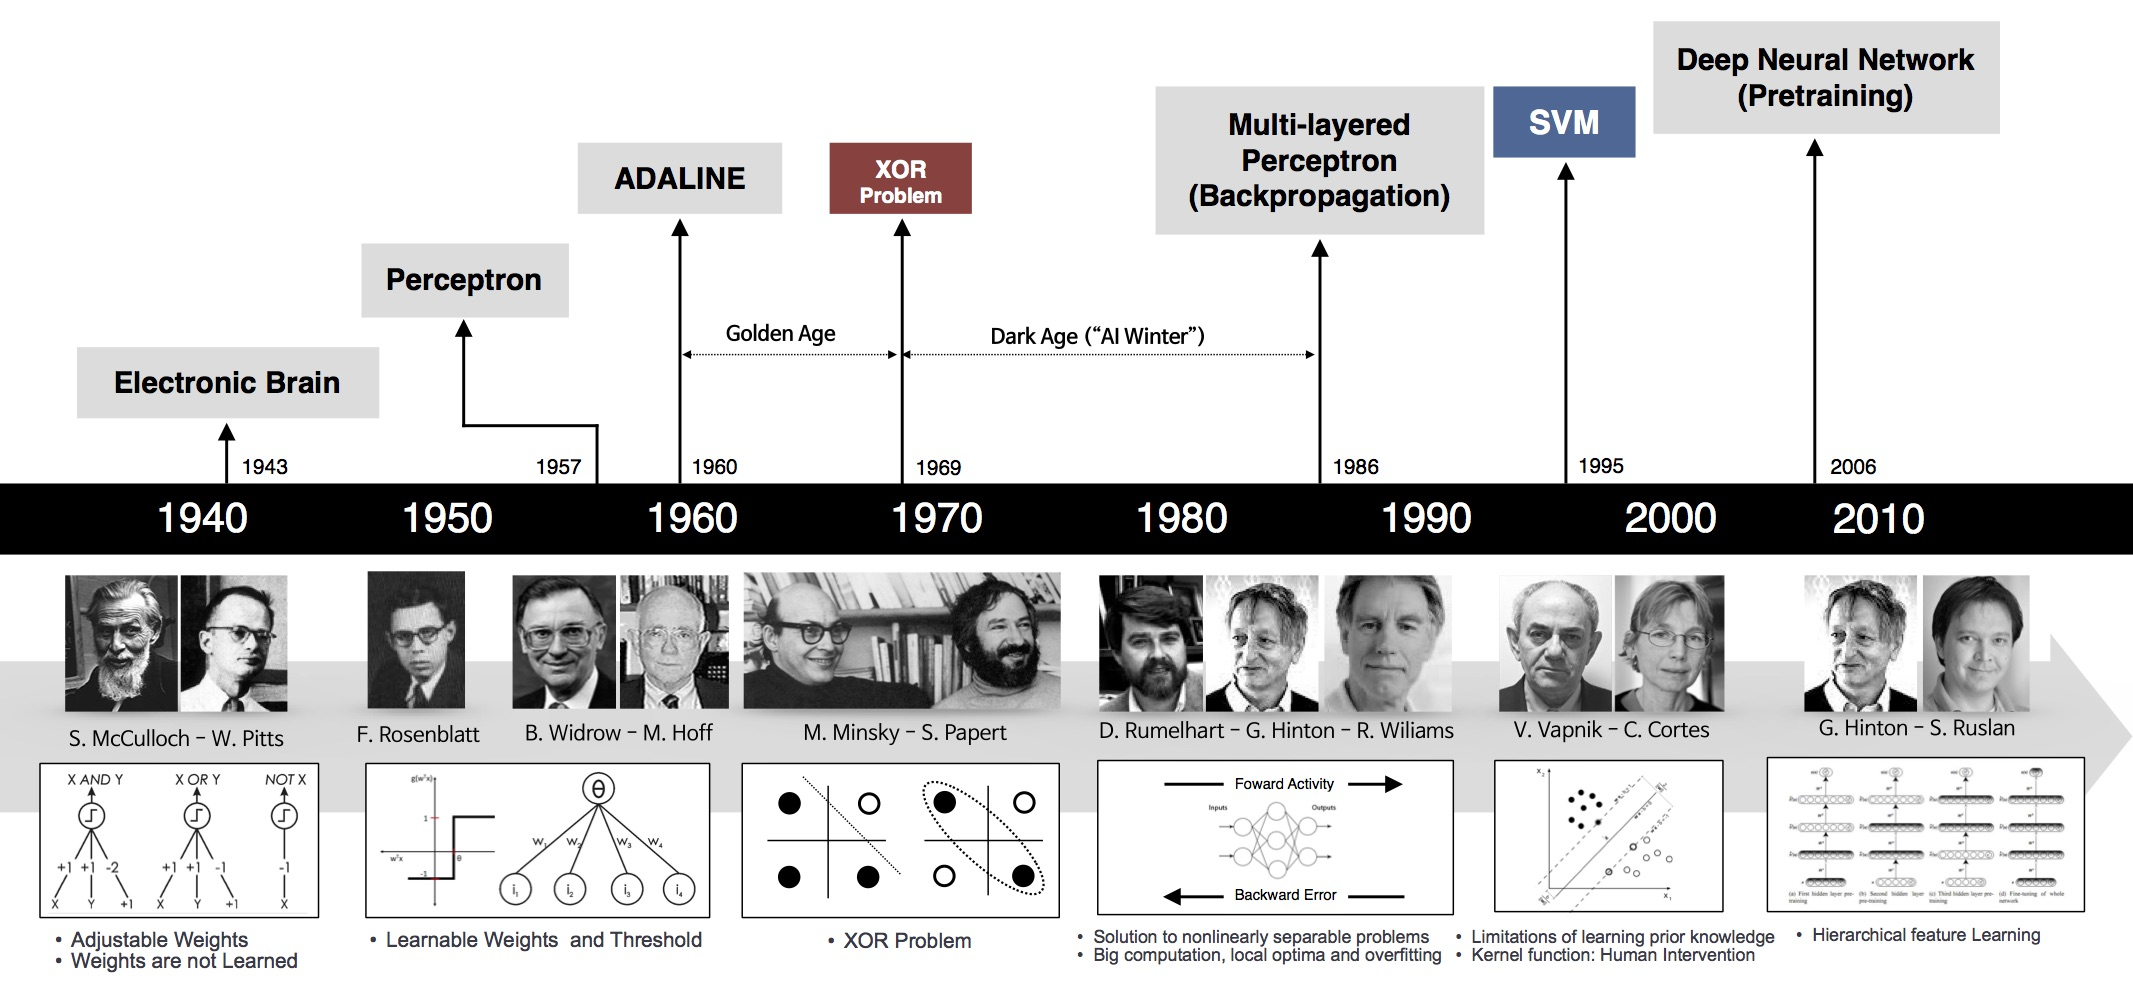
\includegraphics[width=\textwidth]{NN_Timeline.jpg}
  \end{figure}

\end{frame}


%==========================================================================================
\section[Structure of Neural Networks]{Structure of Neural Networks}
%==========================================================================================

%-----------------------------------------------------------------------------------------
\subsection[Single layer perceptron]{Single layer perceptron}
%-----------------------------------------------------------------------------------------

\begin{frame}%[shrink=10]
  \frametitle{Single layer perceptron}

  \begin{figure}
    \centering 
    \resizebox {0.7\columnwidth} {!} {
      
\tikzstyle{inputNode}=[draw,circle,minimum size=10pt,inner sep=0pt]
\tikzstyle{outputNode}=[draw,circle,minimum size=20pt,inner sep=0pt,red,thick,dashed]
\tikzstyle{stateTransition}=[-stealth, thick]

\begin{tikzpicture}
	
	\node[draw,circle,minimum size=26pt,inner sep=0pt] (x) at (0,0) {$\Sigma$ \, $f$};

	\node[inputNode] (x0) at (-2, 1.5)   {$\tiny +1$};
	\node[inputNode] (x1) at (-2, 0.75)  {$\tiny x_1$};
	\node[inputNode] (x2) at (-2, 0)     {$\tiny x_2$};
	\node[inputNode] (x3) at (-2, -0.75) {$\tiny x_3$};
	\node[inputNode] (xn) at (-2, -1.75) {$\tiny x_n$};

	\draw[stateTransition] (x0) to[out=0,in=120] node [midway, sloped, above] {$w_0$} (x);
	\draw[stateTransition] (x1) to[out=0,in=150] node [midway, sloped, above] {$w_1$} (x);
	\draw[stateTransition] (x2) to[out=0,in=180] node [midway, sloped, above] {$w_2$} (x);
	\draw[stateTransition] (x3) to[out=0,in=210] node [midway, sloped, above] {$w_3$} (x);
	\draw[stateTransition] (xn) to[out=0,in=240] node [midway, sloped, above] {$w_n$} (x);
	
	\draw[stateTransition] (x) -- (4,0) node [midway,above] {$f\left(w_0 + \sum\limits_{i=1}^{n}{w_ix_i}\right)$};
	
	\node[outputNode] (y) at (4.5, 0) {$y$};
	
	\draw[dashed] (0,-0.43) -- (0,0.43);
	
	\node (dots) at (-2, -1.15) {$\vdots$};

\end{tikzpicture}
    }
  \end{figure}
  
  \begin{itemize}
    \item \bluebf{$\vec{x} = (x_1, x_2, \cdots, x_n)$ is an input feature vector of length $n$}
    \begin{itemize}
      i.e. the attributes of the data, e.g. voltages
    \end{itemize}
    \item \bluebf{$\vec{w} = (w_1, w_2, \cdots, w_n)$ is the weight vector with $w_0$ reserved as a \textbf{bias}}
    \begin{itemize}
      \item becomes a matrix for multiple layers
    \end{itemize}
    \item \bluebf{$\Sigma$ indicates summation (or matrix mult.): $z = \sum w_i x_i$ ($x_0 = 1$)}
    \item \bluebf{$f$ is the activation function, or non-linearity: $f(z)$}
    \item \alertbf{$y = f(z)$ is the output}
  \end{itemize}
  
\end{frame}

%-----------------------------------------------------------------------------------------

\begin{frame}%[shrink=10]
  \frametitle{Sigmoid as activation function}

  As we discussed, a typical function for a \alertbf{single layer perceptron} is the \textbf{sigmoid}. 

  \begin{figure}
    \centering 
    \resizebox {0.8\columnwidth} {!} {
      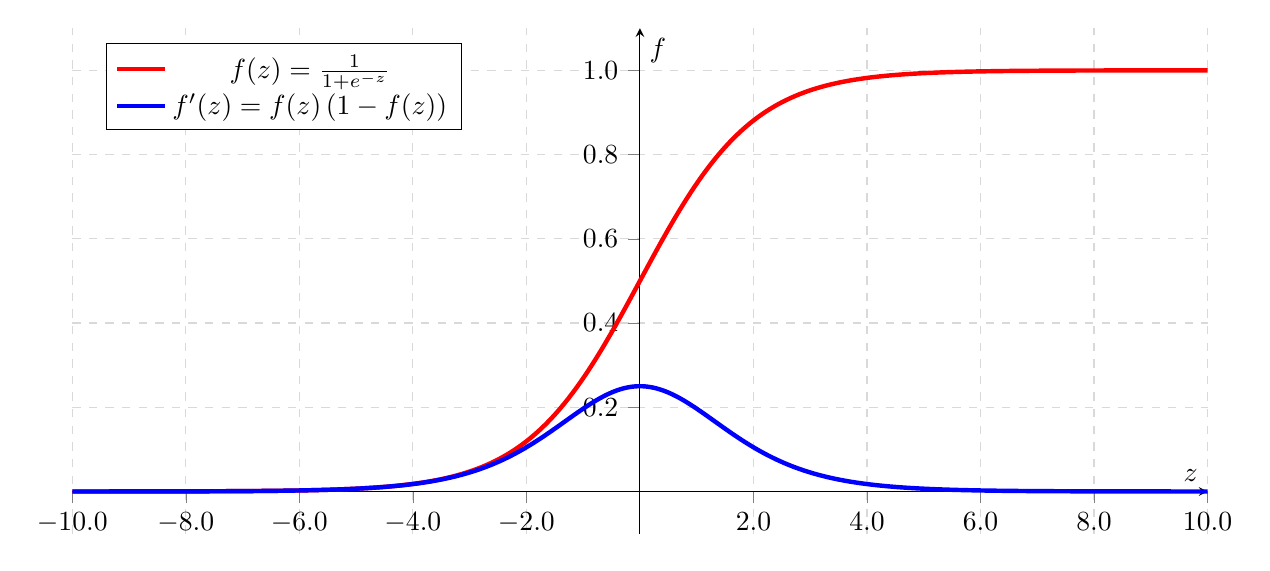
\begin{tikzpicture}
    \begin{axis}[
    	legend pos=north west,
        axis x line=middle,
        axis y line=middle,
        x tick label style={/pgf/number format/fixed,
                            /pgf/number format/fixed zerofill,
                            /pgf/number format/precision=1},
        y tick label style={/pgf/number format/fixed,
                            /pgf/number format/fixed zerofill,
                            /pgf/number format/precision=1},
        grid = major,
        width=16cm,
        height=8cm,
        grid style={dashed, gray!30},
        xmin=-10,     % start the diagram at this x-coordinate
        xmax= 10,    % end   the diagram at this x-coordinate
        ymin= -0.1,     % start the diagram at this y-coordinate
        ymax= 1.1,   % end   the diagram at this y-coordinate
        %axis background/.style={fill=white},
        xlabel=$z$,
        ylabel=$f$,
        tick align=outside,
        enlargelimits=false]
      % plot the stirling-formulae
      \addplot[domain=-10:10, red, ultra thick,samples=500] {1/(1+exp(-x))};
      \addplot[domain=-10:10, blue, ultra thick,samples=500] {exp(-x)/((1+exp(-x))*(1+exp(-x)))};
      \addlegendentry{$f(z)=\frac{1}{1+e^{-z}}$}
      \addlegendentry{$f^{\prime}(z)=f(z)\left(1-f(z)\right)$}
    \end{axis}
\end{tikzpicture}
    }
  \end{figure}
  
  Here, we plot both the function itself, as well as its derivative, since that will be important when evaluating the \bluebf{backpropagation} of weights in order to update the neural network.

\end{frame}

%-----------------------------------------------------------------------------------------
\subsection[Training a single layer perceptron]{Training a single layer perceptron}
%-----------------------------------------------------------------------------------------


\begin{frame}%[shrink=10]
  \frametitle{Training a single layer perceptron}

  \begin{figure}
    \centering 
    \resizebox {0.7\columnwidth} {!} {
      
\tikzstyle{inputNode}=[draw,circle,minimum size=10pt,inner sep=0pt]
\tikzstyle{outputNode}=[draw,circle,minimum size=20pt,inner sep=0pt,red,thick,dashed]
\tikzstyle{stateTransition}=[-stealth, thick]

\begin{tikzpicture}
	
	\node[draw,circle,minimum size=26pt,inner sep=0pt] (x) at (0,0) {$\Sigma$ \, $f$};

	\node[inputNode] (x0) at (-2, 1.5)   {$\tiny +1$};
	\node[inputNode] (x1) at (-2, 0.75)  {$\tiny x_1$};
	\node[inputNode] (x2) at (-2, 0)     {$\tiny x_2$};
	\node[inputNode] (x3) at (-2, -0.75) {$\tiny x_3$};
	\node[inputNode] (xn) at (-2, -1.75) {$\tiny x_n$};

	\draw[stateTransition] (x0) to[out=0,in=120] node [midway, sloped, above] {$w_0$} (x);
	\draw[stateTransition] (x1) to[out=0,in=150] node [midway, sloped, above] {$w_1$} (x);
	\draw[stateTransition] (x2) to[out=0,in=180] node [midway, sloped, above] {$w_2$} (x);
	\draw[stateTransition] (x3) to[out=0,in=210] node [midway, sloped, above] {$w_3$} (x);
	\draw[stateTransition] (xn) to[out=0,in=240] node [midway, sloped, above] {$w_n$} (x);
	
	\draw[stateTransition] (x) -- (4,0) node [midway,above] {$f\left(w_0 + \sum\limits_{i=1}^{n}{w_ix_i}\right)$};
	
	\node[outputNode] (y) at (4.5, 0) {$y$};
	
	\draw[dashed] (0,-0.43) -- (0,0.43);
	
	\node (dots) at (-2, -1.15) {$\vdots$};

\end{tikzpicture}
    }
  \end{figure}
  
  Given $j$ objects $\vec{x}_j$ in dataset, each with \alertbf{known values of $f$}, $d_j$
  \begin{itemize}
    \item \bluebf{Calculate the output:} $y_j = f(\vec{w}\cdot\vec{x}_j)$
    \item \bluebf{Determine the error:} $\epsilon_j = d_j - y_j$
    \item \bluebf{Update the weights:} $w^{\mathrm{new}}_i = w_i + r ( \epsilon_j \cdot \vec{x}_j )_{i}$
  \end{itemize}
  
  Choosing the learning rate $r$ is where the derivative is used. It's not important for the single-layer perceptron, but is \alertbf{essential} for a network.
  
\end{frame}

%-----------------------------------------------------------------------------------------
\subsection[Training a Multi-Layer Perceptron (MLP)]{Training a Multi-Layer Perceptron (MLP)}
%-----------------------------------------------------------------------------------------

\begin{frame}[shrink=20]
  \frametitle{Multi-layer perceptron (MLP)}

  \vspace{-0.8cm}

  \begin{figure}
    \centering 
    \resizebox {\columnwidth} {!} {
      
\tikzstyle{inputNode}=[draw,circle,minimum size=10pt,inner sep=0pt]
\tikzstyle{stateTransition}=[-stealth, thick]

\begin{tikzpicture}
	\node[draw,circle,minimum size=25pt,inner sep=0pt] (x) at (0,0) {$\Sigma$ \, $f$};

    %% Inputs to node
	\node[inputNode] (x0) at (-2, 1.5)   {$\tiny +1$};
	\node[inputNode] (x1) at (-2, 0.75)  {$\tiny x_1$};
	\node[inputNode] (x2) at (-2, 0)     {$\tiny x_2$};
	\node[inputNode] (x3) at (-2, -0.75) {$\tiny x_3$};
	\node[inputNode] (xn) at (-2, -1.75) {$\tiny x_n$};

	\draw[stateTransition] (x0) to[out=0,in=120] node [midway, sloped, above] {$w_0$} (x);
	\draw[stateTransition] (x1) to[out=0,in=150] node [midway, sloped, above] {$w_1$} (x);
	\draw[stateTransition] (x2) to[out=0,in=180] node [midway, sloped, above] {$w_2$} (x);
	\draw[stateTransition] (x3) to[out=0,in=210] node [midway, sloped, above] {$w_3$} (x);
	\draw[stateTransition] (xn) to[out=0,in=240] node [midway, sloped, above] {$w_n$} (x);
	
	\draw[stateTransition] (x) -- (4,0) node [midway,above] {$f\left(w_0 + \sum\limits_{i=1}^{n}{w_ix_i}\right)$};
	
	\draw[dashed] (0,-0.43) -- (0,0.43);
	\node (dots) at (-2, -1.15) {$\vdots$};
	
	% This is the multi-layer graph
	\node[inputNode, thick] (i1) at (6, 0.75) {};
	\node[inputNode, thick] (i2) at (6, 0) {};
	\node[inputNode, thick, label=below:{\small $i$}] (i3) at (6, -0.75) {};
	
	\node[inputNode, thick] (h1) at (8, 1.5) {};
	\node[inputNode, thick] (h2) at (8, 0.75) {};
	\node[inputNode, thick] (h3) at (8, 0) {};
	\node[inputNode, thick] (h4) at (8, -0.75) {};
	\node[inputNode, thick, label=below:{\small $h$}] (h5) at (8, -1.5) {};
	
	\node[inputNode, thick] (o1) at (10, 0.75) {};
	\node[inputNode, thick, label=below:{\small $o$}] (o2) at (10, -0.75) {};
	
	\draw[stateTransition] (5, 0.75) -- node[above] {$I_1$} (i1);
	\draw[stateTransition] (5, 0) -- node[above] {$I_2$} (i2);
	\draw[stateTransition] (5, -0.75) -- node[above] {$I_3$} (i3);
	
	\draw[stateTransition] (i1) -- (h1);
	\draw[stateTransition] (i1) -- (h2);
	\draw[stateTransition] (i1) -- (h3);
	\draw[stateTransition] (i1) -- (h4);
	\draw[stateTransition] (i1) -- (h5);
	\draw[stateTransition] (i2) -- (h1);
	\draw[stateTransition] (i2) -- (h2);
	\draw[stateTransition] (i2) -- (h3);
	\draw[stateTransition] (i2) -- (h4);
	\draw[stateTransition] (i2) -- (h5);
	\draw[stateTransition] (i3) -- (h1);
	\draw[stateTransition] (i3) -- (h2);
	\draw[stateTransition] (i3) -- (h3);
	\draw[stateTransition] (i3) -- (h4);
	\draw[stateTransition] (i3) -- (h5);
	
	\draw[stateTransition] (h1) -- (o1);
	\draw[stateTransition] (h1) -- (o2);
	\draw[stateTransition] (h2) -- (o1);
	\draw[stateTransition] (h2) -- (o2);
	\draw[stateTransition] (h3) -- (o1);
	\draw[stateTransition] (h3) -- (o2);
	\draw[stateTransition] (h4) -- (o1);
	\draw[stateTransition] (h4) -- (o2);
	\draw[stateTransition] (h5) -- (o1);
	\draw[stateTransition] (h5) -- (o2);
	
	\node[above=of i1, align=center] (l1)       {Input \\ layer};
	\node[right=2.3em of l1, align=center] (l2) {Hidden \\ layer};
	\node[right=2.3em of l2, align=center] (l3) {Output \\ layer};
	
	\draw[stateTransition] (o1) -- node[above] {$O_1$} (11, 0.75);
	\draw[stateTransition] (o2) -- node[above] {$O_2$} (11, -0.75);
	
	\path[dashed, double, ultra thick, gray] (x.north) edge[bend left=0]  (h5.north);
	\path[dashed, double, ultra thick, gray] (x.south) edge[bend right=0] (h5.south);
\end{tikzpicture}
    }
  \end{figure}
  
  Given $j$ objects $\vec{I}_j$ in dataset, each with features $\vec{I} = (I_1, I_2, \cdots, I_n)$ and \alertbf{known outputs $\vec{d}_j$ at each output node $o$}, $\vec{d} = (d_1, d_2, \cdots, d_o)$
  \begin{itemize}
    \item \bluebf{Calculate the $h$ outputs of hidden layer:} $v_h = f(\sum_i w_{ih} I_i)$
    \item \bluebf{Calculate the $o$ outputs of output layer:} $y_o = f(\sum_h w_{ho} v_h)$
    \item \bluebf{Determine the error at output each node $o$:} $\epsilon_o = d_o - y_o$
    \item \bluebf{Determine the total error for data object $j$:} $\mathcal{E}_j = \frac{1}{2} \sum_o \epsilon_o^{2}$
    \item \bluebf{Determine change in weights for output neuron $y_o$:} $\Delta w_{oh}=-\eta {\frac {\partial {\mathcal{E}}}{\partial z_{o}}}v_{h} = \eta \epsilon_o \, f^{\prime}(z_{o})$
  \end{itemize}
    
\end{frame}

%-----------------------------------------------------------------------------------------

\begin{frame}[shrink=20]
  \frametitle{LeCun, Bengio, Hinton, ``Deep learning''}
  \framesubtitle{\href{https://www.nature.com/articles/nature14539\#f1}{Nature volume 521, pages 436-444 (28 May 2015)} }

  \vspace{-0.3cm}

  \begin{figure}
    \centering 
    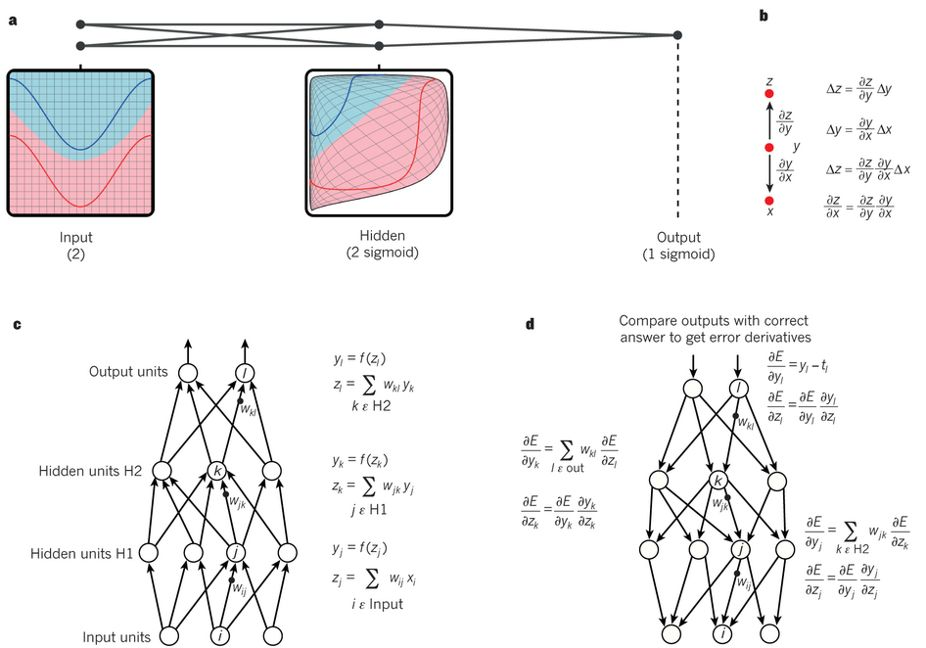
\includegraphics[width=\textwidth]{BackPropagation-LeCun-Nature.jpg}
  \end{figure}
  

    
\end{frame}

%-----------------------------------------------------------------------------------------

%\begin{frame}%[shrink=20]
%
%  \begin{figure}
%    \centering 
%    \resizebox {0.7\columnwidth} {!} {
%      
\tikzstyle{inputNode}=[draw,circle,minimum size=10pt,inner sep=0pt]
\tikzstyle{outputNode}=[draw,circle,minimum size=20pt,inner sep=0pt,red,thick,dashed]
\tikzstyle{stateTransition}=[-stealth, thick]

\begin{tikzpicture}
	
	\node[draw,circle,minimum size=26pt,inner sep=0pt] (x) at (0,0) {$\Sigma$ \, $f$};

	\node[inputNode] (x0) at (-2, 1.20)  {$\tiny +1$};
	\node[inputNode] (x1) at (-2, 0.40)  {$\tiny x_1$};
	\node[inputNode] (x2) at (-2,-0.40)  {$\tiny x_2$};
	\node[inputNode] (x3) at (-2,-1.20)  {$\tiny x_3$};

	\draw[stateTransition] (x0) to[out=0,in=120] node [midway, sloped, above] {$w_0$} (x);
	\draw[stateTransition] (x1) to[out=0,in=150] node [midway, sloped, above] {$w_1$} (x);
	\draw[stateTransition] (x2) to[out=0,in=210] node [midway, sloped, above] {$w_2$} (x);
	\draw[stateTransition] (x3) to[out=0,in=240] node [midway, sloped, above] {$w_3$} (x);
	
	\draw[stateTransition] (x) -- (4,0) node [midway,above] {$f\left(w_0 + \sum\limits_{i=1}^{n}{w_ix_i}\right)$};
	
	\node[outputNode] (y) at (4.5, 0) {$y$};
	
	\draw[dashed] (0,-0.43) -- (0,0.43);
	

\end{tikzpicture}
%    }
%  \end{figure}
%
%\end{frame}

  
%==========================================================================================
%==========================================================================================
\end{document}
